\chapter{Uvod}
\thispagestyle{fancy}
\pagenumbering{arabic}
Motivacija za raziskavo je bilo ugotoviti do kakšne mere je mogoča razpoznavanje gibanja v živo na osnovi analize možganske aktivnosti z EEG meritvami. Najprej smo podatke iz prosto dostopne zbirke podatkov s pomočjo knjižnice EEGLAB razdelili na nekaj različno dolgih epoh po dogodkih in jim zožili frekvenčne pasove. Iz vsake pridobljene zbirke podatkov smo pridobili matrike povezljivosti Grangerjevega indexa vzročnosti in matrike povezljivosti kompleksnega Pearsonovega korelacijskega koeficienta. Na pridobljenih podatkih smo naučili nevronsko mrežo. Iz pridobljenih rezultatov smo se odločili za nadaljevanje razvoja na zbirki, ki je obetala najboljšo točnost. Da bi omogočili delovanje v realnem času smo sami implementirali nekaj že obstoječih funkcij iz knjižnice. Posneli smo podatke na Cognionics Quick-20 in dodatno naučili nevronsko mrežo na naših podatkih za boljšo klasifikacijo.
\newpage
\section{Elektroencefalografija}
Elektroencefalografija(EEG) je metoda za merjenje možganske električne aktivnosti. Meri električne potenciale na površini temena ki jih deloma generira možganska aktivnost. V zadnjem stoletju so znanstveniki s pomočjo EEG pridobili vpogled v različne nevrološke bolezni. V zadnjem času pa se pojavlja interes v modeliranju eeg signalov in uporabo le teh za nadzor fizičnih naprav. EEG signali so običajno razdeljeni v območja ki odražajo različne spektralne vrhove. Ta območja so običajno določena kot delta (1-4 Hz), theta (4-8 Hz), alpha (8-13 Hz), beta (13-20 Hz), in gamma (<20 Hz). 
 \cite{nunezElectroencephalographyEEGNeurophysics2016}
 \begin{figure}[h!]
    \begin{center}
    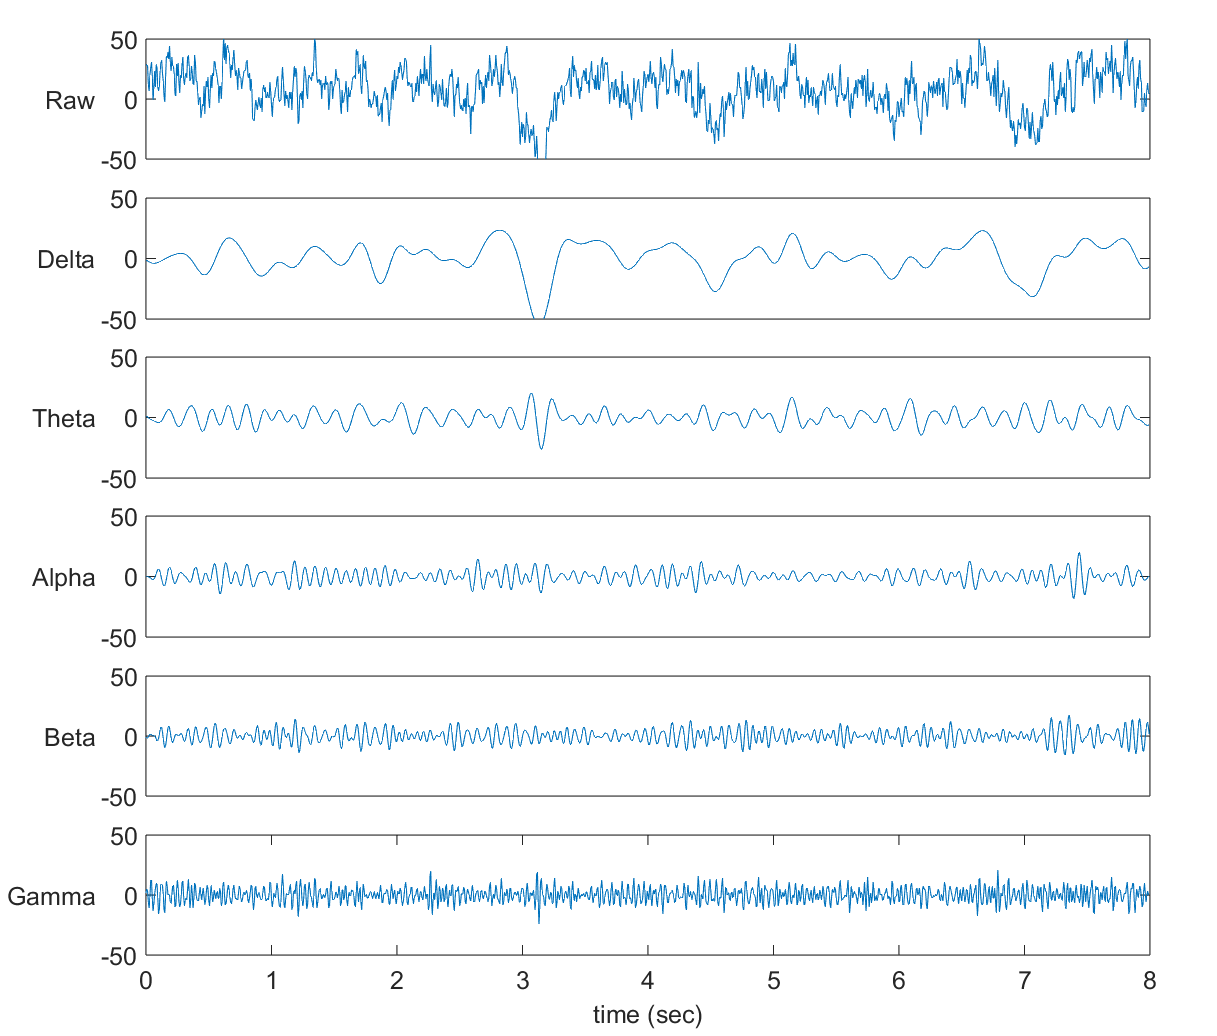
\includegraphics[width=1\linewidth]{slike/EEGSignals.png}
    \end{center}
    \caption{Prvih 8 sekund EEG signala elektrode C3, osebe S001 serije R03. Od zgoraj navzdol po področjih: vsa skupaj, delta, theta, alpha, beta, gamma.}
    \end{figure}


\subsection{Mednarodni sitem 10-20 pozicioniranja elektrod}
Mednarodni sistem 10-20 standardizira mesta elektrod tako, da so te  nameščene v mrežo od naziona do iniona ter od desnega do levega sluhovoda v presledkih 10 in 20 odstotkov razdalje. Vsaka elektroda je označena z črko lokacijo: T-Temporal, F-Frontal, P-Parietal, C-Central in O-Occipital, ter z črko z za elektrode na sredini glave, lihimi številkami za levo polovico glave in sodimi za desno. \cite{klemTentwentyElectrodeSystem1999}
\begin{figure}[h!]
    \begin{center}
    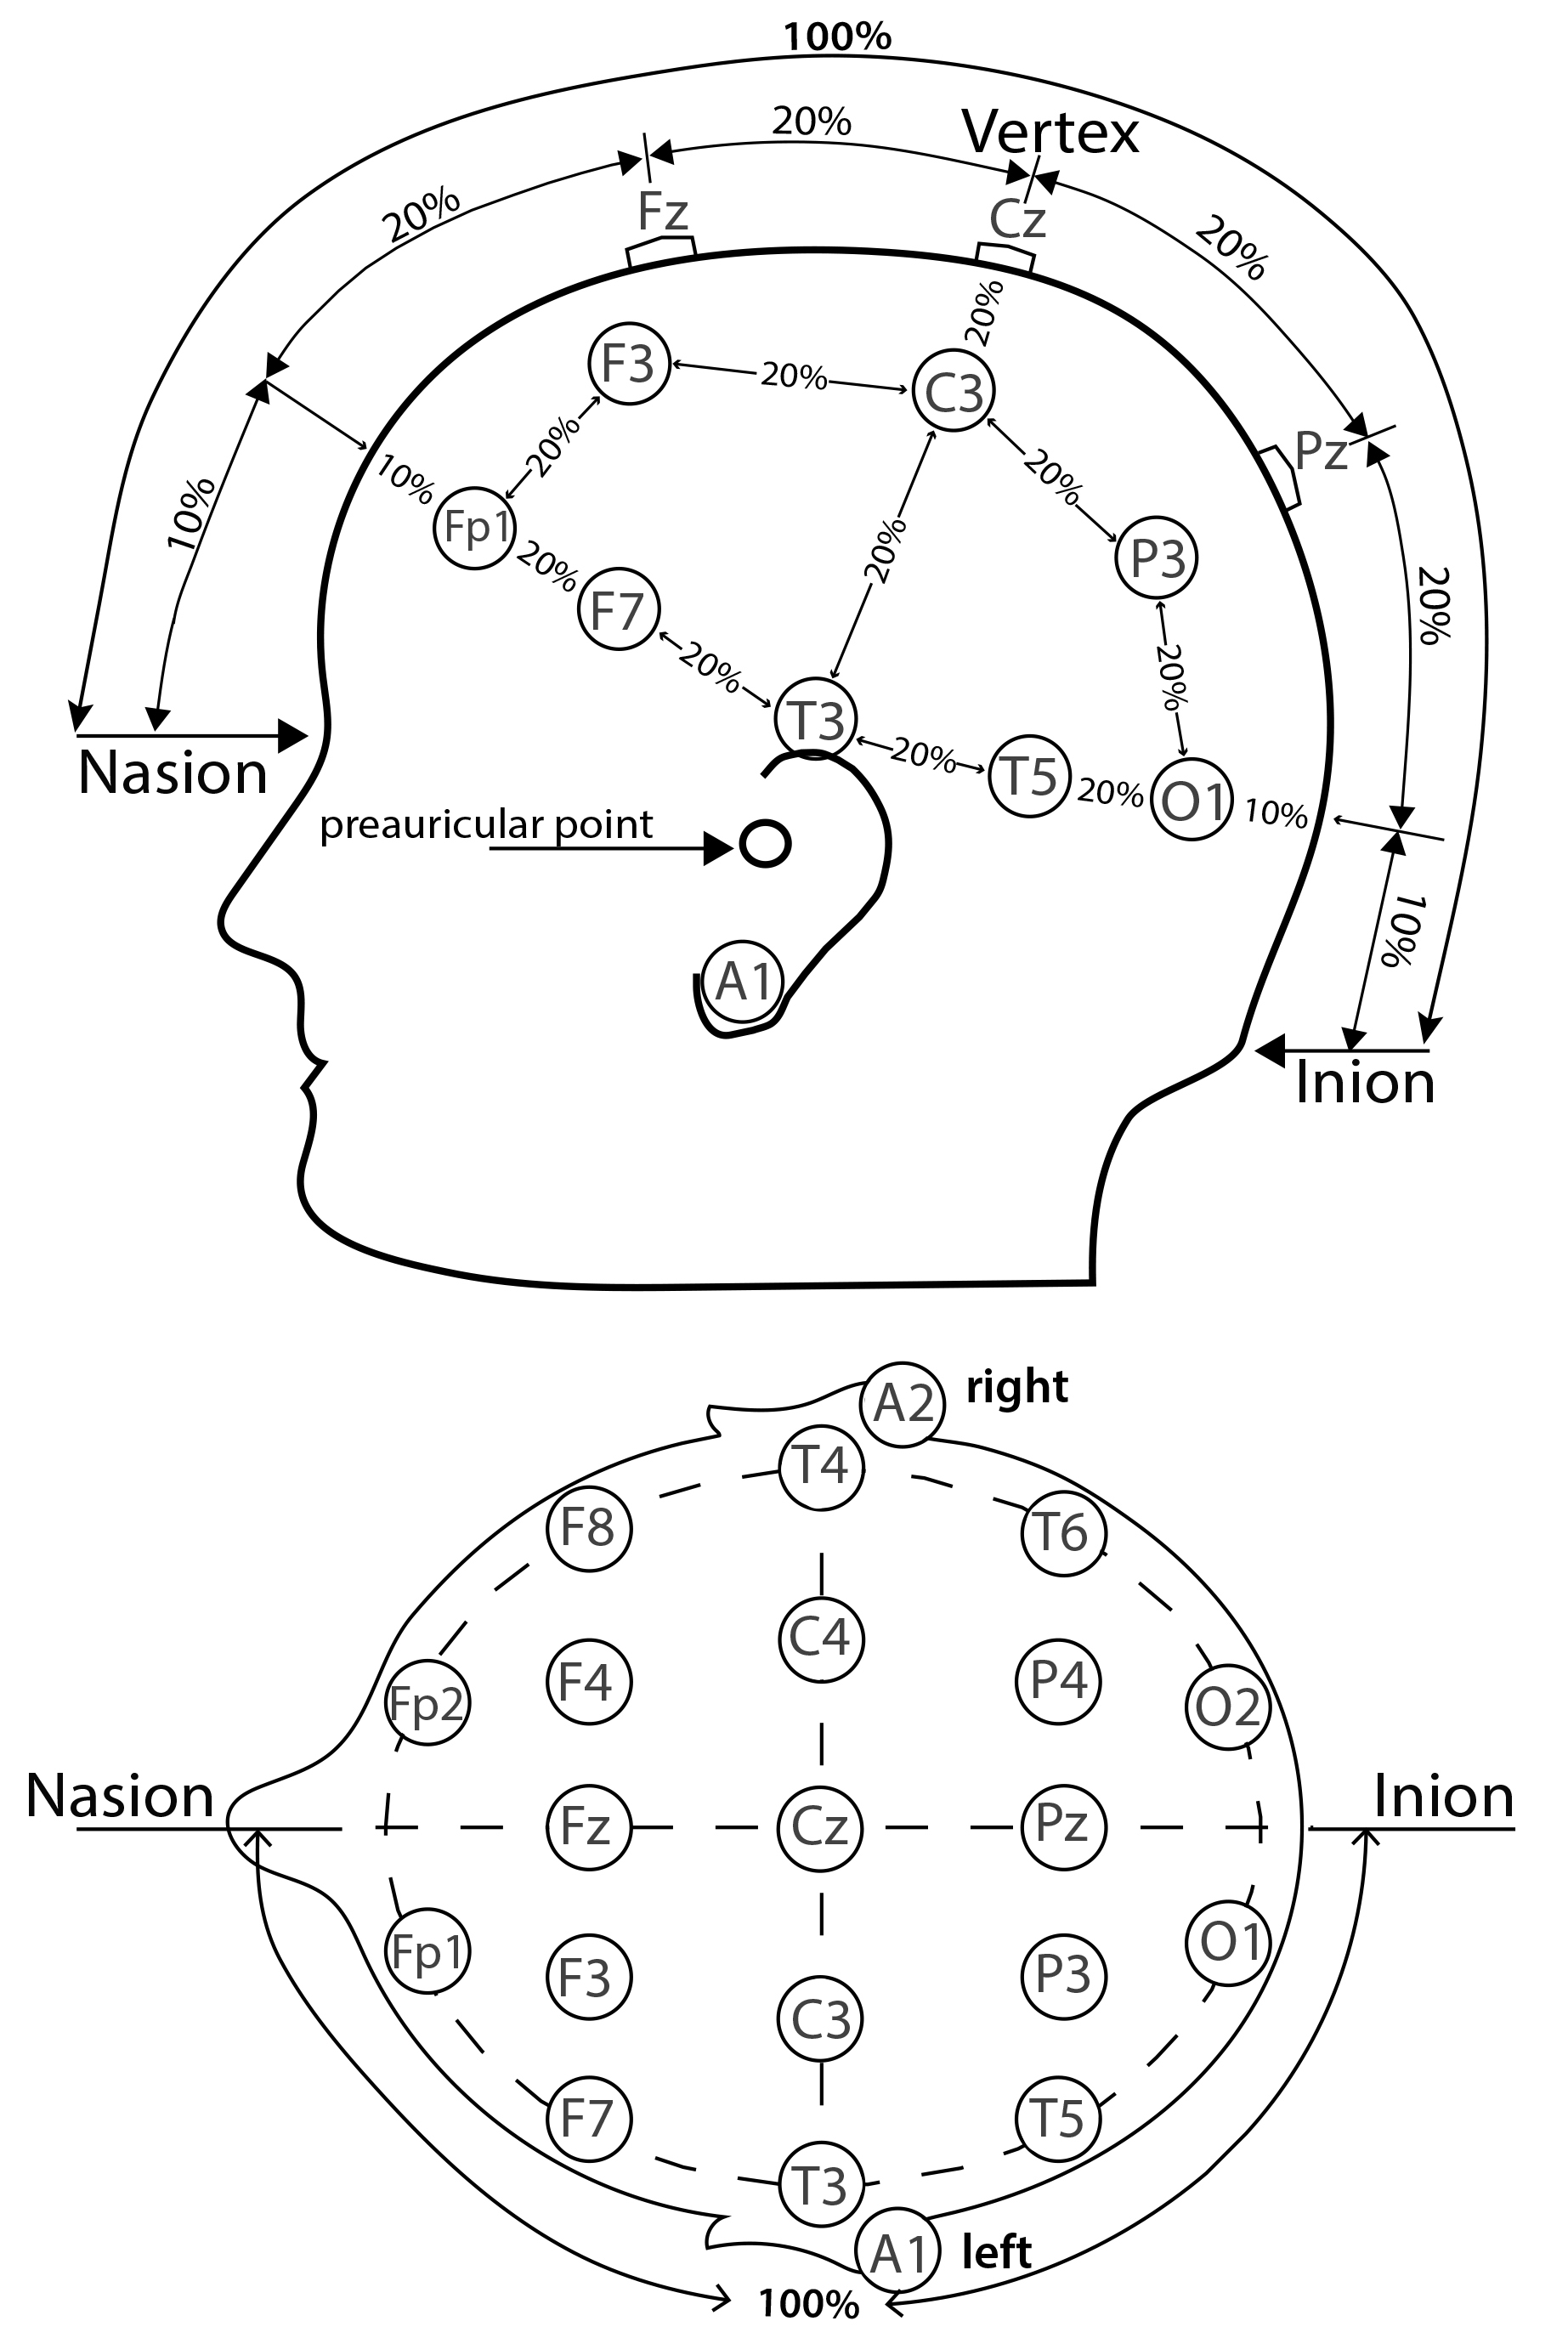
\includegraphics[width=0.7\linewidth]{slike/1020-diagram1.jpg}
    \end{center}
    \caption{Prikaz pozicije elektrod po mednarodnem sitemu 10-20. Nameščene v mrežo od naziona do iniona in od levevega do desnega sluhovoda v presledkih 10 in 20 odstotkov. \cite{ElectrodeArrangementAccording}}
    \end{figure}


\subsection{Cognionics Quick-20}
Cognionics Quick-20 je brezžična suha EEG naprava za raziskovalne namene. Ima 21 elektrod postavljenih po mednarodnem sitemu 10-20 za pozicionire elektrod. Naparava je suhega tipa kar pomeni, da pri uporabi elektrode ne potrebujejo gela. Suhi tipi naprav so v primerjavi z mokrimi enostavni in udobni za uporabu in omogočajo hitro nastavitev. Naprava je brezžična, z računalnikom jo povežemo preko USB vmesnika. \cite{DryEEGHeadset}

\begin{figure}[h!]
    \begin{center}
    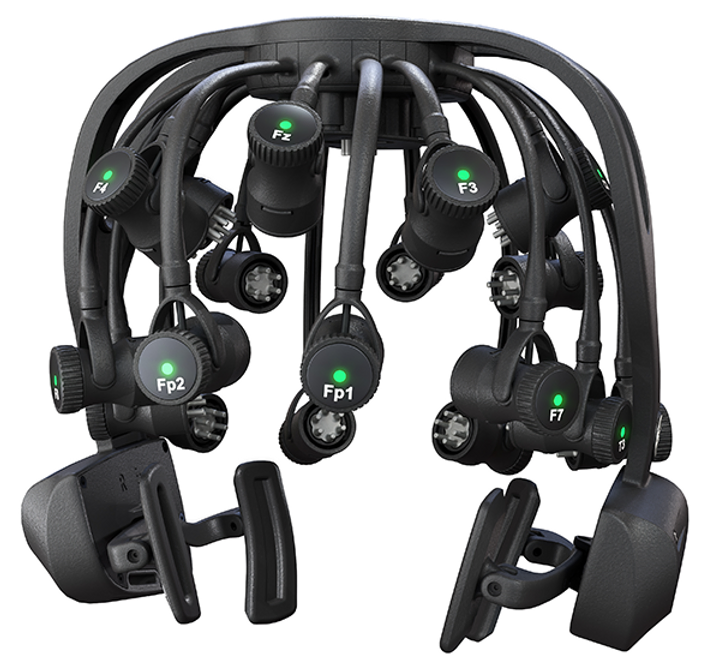
\includegraphics[width=0.5\linewidth]{slike/Cognionics Quick-20.png}
    \end{center}
    \caption{EEG naprava Cognionics Quick-20. \cite{DryEEGHeadset}}
    \end{figure}

\section{Povezljivost}
Povezljivost se nananaša na vzorce nastale zaradi anatomskih povezav možganov, statistične odvisnosti ali interakcij med posameznimi deli možganov.  Enote med katerimi se meri povezljivost so lahko različne: posamezni nevroni, nevronske populacije, v našem primeru pa regije možganske skorje. Možganska aktivnost je omejena s povezljivostjo, le ta pa je zato ključnega pomena za razumevanje delovanja možganov. V grobem poznamo dve vrsti povezljivosti: strukturno in funkcijsko. Strukturna povezanost se nanaša na to kako so deli možganov med seboj fizično povezani. Funkcijska povezljivost pa se nanaša na to kako različni deli možganov med seboj komunicrajo oziroma sodelujejo.\cite{spornsBrainConnectivity2007} Funkcijsko povezljivost lahko nadaljno delimo na usmerjeno in neusmerjeno. V našem primeru je metoda Grangerjevega indexa vzročnosti usmerjena saj je vpliv elektrode $A$ na elektrodo $B$ drugačen kot vpliv elektrode $B$ na elektrodo $A$. Metoda kompleksnega Pearsonovega korelacijskega koeficienta pa je neusmerjena saj nam njegova vrednost pove le o povezanosti para elektrod.
